\section{平动和转动}\label{sec:10.02}

上节中,我们论证了刚体具有$ 6 $个自由度,即描写刚体的几何
位形需要$ 6 $个独立坐标。另一方面,选取哪$ 6 $个坐标是完全任意
的。选取什么样的坐标能使我们对刚体的描写更方便呢?为此,
我们来研究刚体运动的特征。

刚体的一种最简单的运动形式是平动。在平动中,刚体中任
% 288.jpg
\clearpage\noindent
何两点之间的连线的方向总是保持不变;刚体中各点都具有同样
的速度,并且运动轨迹的形状也都相同(图\ref{fig:10.06}) 。

\begin{figure}[h]
  \centering
  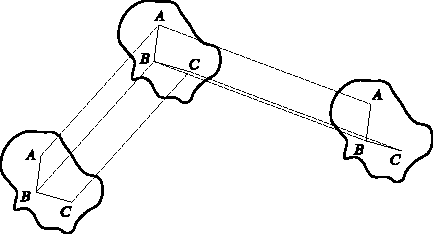
\includegraphics{figure/fig10.06}
  \caption{刚体的平动}
  \label{fig:10.06}
\end{figure}

刚体的另一种最简单的运动形式是绕固定轴的转动。在转动
\begin{wrapfigure}[7]{l}{13em}
  \centering
  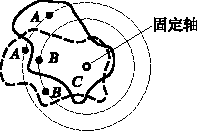
\includegraphics{figure/fig10.07}
  \caption{刚体绕固定轴的转动}
  \label{fig:10.07}
\end{wrapfigure}
时,刚体中各点的轨迹都是在垂
直于转动轴的平面内的圆(\ref{fig:10.07})。

下面我们来证明一个重要的
论断:刚体的任何运动都可以归
结为平动和转动的迭加。举例说,
如图108所示的物体从位置$ A _ { 1 } $移
到位置 $ A _ { 2 } $ 。这个运动可以按下述方式加以分解。设刚体先从 $ A _ { 1 } $ 平
动到$ A' $,这时刚体上的$ O $点已经移到终点位置。然后再将刚体绕点
$ O $转动角$ \Delta \varphi $,则刚体就完全移到了终点位置$ A_2 $。

上述分解表明,从$ A_1 $到$ A_2 $的运动,可以视为从$ A_1 $到$ A' $的平动及
从$ A' $到 $ A _ { 2 } $ 的转动的迭加。显然,在进行上述分解时,对点$ O $的选
取是任意的。我们可以让刚体先从$ A_1 $平动到 $ A ^ {\prime \prime } $的位置,这时另一
点$ O' $已经移到终位置,然后再将刚体绕$ O' $转动而达到位置$ A _ { 2 } $。因
此,从$ A _ { 1 } $到$ A_2 $的运动,可以按多种不同的方式加以分解,即分解% 289.jpg
成平动和转动的选加的方式不是唯一的。
\begin{figure}[h]
  \centering
  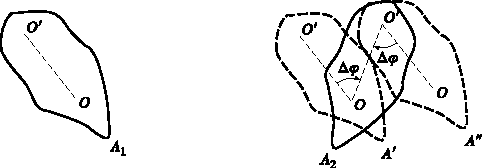
\includegraphics{figure/fig10.08}
  \caption{刚体运动的分解}
  \label{fig:10.08}
\end{figure}%
但重要的是:在不同的
分解方式中转动的角度是一样的,$ A' $到$ A_2 $的转角与$ A'' $到$ A_2 $的转角都等于$ \Delta \varphi $,且方向也一样,都是顺时针转动;而相应的平动路程
是不一样的,$ A $到$ A'' $的路程与$ A $到$ A'' $的路程是不相同的。

现在举例分析一下车轮在地面上沿直线的滚动,如图109所
示。现在平动是一维的,转动轴的方向也是确定的,故转动也是
一维的,所以仅需要两个独立坐标就可描写车轮的滚动问题。所
谓纯滚动,是车轮前进的$ \Delta x $就等于车轮滚过的弧长$\wideparen{\Delta s}$(图\ref{fig:10.09})
即
\begin{equation*}
  \Delta x = \wideparen{\Delta s}
\end{equation*}
\begin{align*}
  \beforetext{又} \wideparen{\Delta s} = r _ { 0 } \Delta \varphi
\end{align*}
\begin{align*}
  \beforetext{所以} \Delta x = r _ { 0 } \Delta \varphi
\end{align*}
\begin{figure}[h]
  \centering
  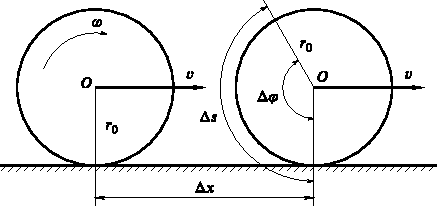
\includegraphics{figure/fig10.09}
  \caption{车轮的滚动}
  \label{fig:10.09}
  \vspace{-0.8em}
\end{figure}

% 290.jpg
\clearpage\noindent
不难断定,在滚动中只有车轮中心$ O $的运动轨迹是直线,其他各
点的轨迹都是曲线,即所谓旋转轮线。我们选$ O $作为基点,如果
车轮在$ \Delta t $时间内位移为$ \Delta x $,则$ O $点的速度为
\begin{equation*}
  \begin{split}
    v _ { 0 } &= \lim_{ \Delta t \to 0 } \frac { \Delta x } { \Delta t} \\
    &= r_ { 0 } \lim_{ \Delta t \to 0 } \frac { \Delta \varphi } { \Delta t } \\
    &= r _ { 0 } \omega
  \end{split}
\end{equation*}
这就是车轮的平动速度。现在,车轮的运动分解为以$ O $点为基点
的平动,其速度为$ v _ { 0 } $ 以及绕$ O $的转动,其角速度为$ 0 $。车轮上任
何一点的速度都是这两种运动速度的合成。

我们来求车轮的垂直于地面的直径上各点的速度。高于$ O $点
的各点,平动速度方向与转动速度方向一致。所以合速度为
\begin{equation}\label{eqn:10.02.01}
  v = v _ { 0 } + r \omega
\end{equation}
其中$ r $是该点与$ O $的距离,对低于$ O $的各点,转动速度方向与平动
速度方向相反,所以合速度为
\begin{equation}\label{eqn:10.02.02}
  v = v _ { 0 } - r \omega
\end{equation}
\begin{wrapfigure}[8]{r}{13em}
  \vspace{-0.8em}
  \centering
  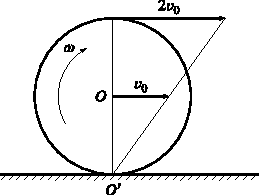
\includegraphics{figure/fig10.10}
  \caption{车轮各点的速度}
  \label{fig:10.10}
\end{wrapfigure}
图\ref{fig:10.10} 中,根据式\eqref{eqn:10.02.01}及式
\eqref{eqn:10.02.01}画出了垂直于地面的直
径上各点的合速度。车轮的最高
点速度最大,比车轮中心速度高
一倍。车轮与地面接触处速度为
零。也就是说,在纯滚动的运动
中,车轮与地面相接触处,总是
相对静止的。

我们知道一物体在另一物体表面滑动时,总有摩擦力,要克
服摩擦力作功就导致损耗能量。对于纯滚动,接触处相对静止,是
静摩擦力一个力作功的功率为$ \vec{F} \cdot \vec{v} $,现在接触处速度为零,所
% 291.jpg
以此时摩擦力不作功。这就是绝大多数交通工具都采用滚动而不
采用滑动的原因。

图\ref{fig:10.10} 还告诉我们,也可以将车轮在该瞬时的运动看成是绕
$ O' $点(车轮与地面接触点)的转动,即过$ O $点作垂直于车轮平面的
转动轴,绕这个轴的角速度同样为$ \omega $。对于过$ O $点或$ O' $点的轴来
说,刚体的角速度都相同,这个性质可以称为角速度的绝对性。

这个结果具有普遍性。一般来说,刚体的任何运动都可以分
解为平动及转动。选定刚体上某点$ O $作为基点,刚体的平动就是
整个刚体跟随基点$ O $的运动,刚体的转动就是围绕通过$ O $点的轴的
运动。这时,刚体的平动速度依赖于对基点$ O $的选择。选择不同
的基点,平动速度就不同;而转动角速度则与基点的选择无关,
不管选择在刚体上任何一点$ O $,角速度矢量的方向及大小都不变
在这个意义上,我们说刚体的角速度具有绝对性。

\begin{figure}[h]
  \centering
  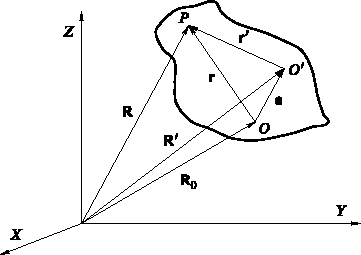
\includegraphics{figure/fig10.11}
  \caption{刚体的角速度的绝对性}
  \label{fig:10.11}
\end{figure}

现在我们来证明上述的论断。图\ref{fig:10.11}表示一个刚体相对于坐
标系K的位形,$ O $及$ P $是刚体上的两点。它们的位置矢量分别是
$ \vec{R}_0 $及$\vec{R}$。显然,$ O $及$ P $相对于$ K $的速度分别为
\begin{equation}\label{eqn:10.02.03}
  \vec{V} = \frac { \dif \vec{R} _ { 0 } } { \dif t } \quad \text{及} \quad \vec{v} = \frac { \dif \vec{R} } { \dif t }
\end{equation}
% 292.jpg
另一方面,$ P $相对于$ O $点的位置矢量为$ \vec{r} $,$ P $相对于$ O $的速度为
\begin{equation}\label{eqn:10.02.04}
  \vec{v} ^ { \prime } = \frac { \dif \vec{r} } { \dif t }
\end{equation}
若选择$ O $为基点,则$ P $相对于$ O $的速度可以表示成
\begin{equation}\label{eqn:10.02.05}
  \vec{v} ^ { \prime } = \vec{\omega} \times \vec{r}
\end{equation}
其中$ \omega $是刚体绕过$ O $点的轴的角速度。由速度合成的运动学,可
知
\begin{equation}\label{eqn:10.02.06}
  \begin{split}
    \vec{v} &= \vec{V} + \vec{v} ^ { \prime } \\
    &= \vec{V} + \vec{\omega } \times \vec{r}
  \end{split}
\end{equation}
如果不选$ O $作为基点,而选$ O' $点,$ O' $点的坐标为$ \vec{R}' $,$ P $相对于$ O' $点
的位置矢量为$\vec{r}'$,则类似于式\eqref{eqn:10.02.06},可以推得
\begin{equation}\label{eqn:10.02.07}
  \vec{v} = \vec{V} ^ { \prime } + \vec{\omega} ^ { \prime } \times \vec{r} ^ { \prime }
\end{equation}
其中$ \vec{V} ^ { \prime } = \dif \vec{R} ^ { \prime } / \dif t $ ,是$ O' $相对于坐标系$ K $的速度;$ \vec{\omega} ^ { \prime } $是刚体绕过点$ O' $
的轴的角速度。

如果$ O' $相对于$ O $的位置矢量为$ \vec{a} $,则有
\begin{equation}\label{eqn:10.02.08}
  \vec{r} = \vec{r} ^ { \prime } + \vec{a}
\end{equation}
将上式代入式\eqref{eqn:10.02.06},得到
\begin{equation}\label{eqn:10.02.09}
  \vec{v} = \vec{V} + \vec{\omega} \times \vec{a} + \vec{\omega} \times \vec{r} ^ { \prime }
\end{equation}
然而, $ \vec{V} + \vec{\omega} \times \vec{a} $正是$ O' $点相对于坐标系$ K $的速度,即
\begin{equation}\label{eqn:10.02.10}
  \vec{V} ^ { \prime } = \vec{V} + \vec{\omega} \times \vec{a }
\end{equation}
由此,式\eqref{eqn:10.02.09}成为
\begin{equation}\label{eqn:10.02.11}
  \vec{v} = \vec{V} ^ { \prime } + \vec{\omega} \times \vec{r} ^ { \prime }
\end{equation}
比较式\eqref{eqn:10.02.07}与式\eqref{eqn:10.02.11},立即得到
\begin{equation}\label{eqn:10.02.12}
  \vec{\omega} = \vec{\omega} ^ { \prime }
\end{equation}
这样,我们就证明了刚体的转动角速度的绝对性。
